%!TEX encoding = UTF-8 Unicode
\documentclass[french, a4paper, 12pt]{article}



%% Langue et compilation

\usepackage[utf8]{inputenc}
\usepackage[T1]{fontenc}
\usepackage[french]{babel}

%% LISTE DES PACKAGES

\usepackage{mathtools}     % package de base pour les maths
\usepackage{amsmath}       % mathematical type-setting
\usepackage{amssymb}       % symbols speciaux pour les maths
\usepackage{textcomp}      % symboles speciaux pour el text
\usepackage{gensymb}       % commandes generiques \degree etc...
\usepackage{tikz}          % package graphique
\usepackage{wrapfig}       % pour entourer a cote d'une figure
\usepackage{color}         % package des couleurs
\usepackage{xcolor}        % autre package pour les couleurs
\usepackage{pgfplots}      % pacakge pour creer des graph
\usepackage{epsfig}        % permet d'inclure des graph en .eps
\usepackage{graphicx}      % arguments dans includegraphics
\usepackage{pdfpages}      % permet d'insérer des pages pdf dans le document
\usepackage{subfig}        % permet de creer des sous-figure
\usepackage{pst-all}       % utile pour certaines figures en pstricks
\usepackage{lipsum}        % package qui permet de faire des essais
\usepackage{array}         % permet de faire des tableaux
\usepackage{multicol}      % plusieurs colonnes sur une page
\usepackage{enumitem}      % pro­vides user con­trol: enumerate, itemize and description
\usepackage{hyperref}      % permet de creer des hyperliens dans le document
\usepackage{lscape}        % permet de mettre une page en mode paysage
\usepackage{lmodern}       % permet d'avoir certains "fonts" de bonen qualite
\usepackage{fancyhdr}      % Permet de mettre des informations en hau et en bas de page      
\usepackage[framemethod=tikz]{mdframed} % breakable frames and coloured boxes
\usepackage[top=1.5cm, bottom=1.5cm, left=2.5cm, right=2.5cm]{geometry} % donne les marges
\usepackage[font=normalsize, labelfont=bf,labelsep=endash, figurename=Fig.]{caption} % permet de changer les legendes des figures
\usepackage{lewis}
\usepackage{bohr}
\usepackage{chemfig}
\usepackage{chemist}

%% LIBRAIRIES

\usetikzlibrary{plotmarks} % librairie pour les graphes
\usetikzlibrary{patterns}  % necessaire pour certaines choses predefinies sur tikz
\usetikzlibrary{shadows}   % ombres des encadres
\usetikzlibrary{backgrounds} % arriere plan des encadres


%% MISE EN PAGE

\pagestyle{fancy}     % Défini le style de la page

\renewcommand{\headrulewidth}{1pt}      % largeur du trait en haut de la page
\fancyhead[L]{Seconde générale}         % info coin haut gauche
\fancyhead[R]{Lycée Jean Guéhenno}  % info coin haut droit

% bas de la page
\renewcommand{\footrulewidth}{1pt}      % largeur du trait en bas de la page
\fancyfoot[L]{G. \bsc{LE DOUDIC}}  % info coin bas gauche
\fancyfoot[R]{TP 4 : Famille chimique}                         % info coin bas droit


\setlength{\columnseprule}{1pt} 
\setlength{\columnsep}{30pt}



%% NOUVELLES COMMANDES 

\DeclareMathOperator{\e}{e} % permet d'ecrire l'exponentielle usuellement


\newcommand{\gap}{\vspace{0.15cm}}   % defini une commande pour sauter des lignes
\renewcommand{\vec}{\overrightarrow} % permet d'avoir une fleche qui recouvre tout le vecteur
\newcommand{\bi}{\begin{itemize}}    % begin itemize
\newcommand{\ei}{\end{itemize}}      % end itemize
\newcommand{\bc}{\begin{center}}     % begin center
\newcommand{\ec}{\end{center}}       % end center
\newcommand\opacity{1}               % opacity 
\pgfsetfillopacity{\opacity}

\newcommand*\Laplace{\mathop{}\!\mathbin\bigtriangleup} % symbole de Laplace

\frenchbsetup{StandardItemLabels=true} % je ne sais plus

\newcommand{\smallO}[1]{\ensuremath{\mathop{}\mathopen{}o\mathopen{}\left(#1\right)}} % petit o

\newcommand{\cit}{\color{blue}\cite} % permet d'avoir les citations de couleur bleues
\newcommand{\bib}{\color{black}\bibitem} % paragraphe biblio en noir et blanc
\newcommand{\bthebiblio}{\color{black} \begin{thebibliography}} % idem necessaire sinon bug a cause de la couleur
\newcommand{\ethebiblio}{\color{black} \end{thebibliography}}   % idem
%%% TIKZ


%% COULEURS 


\definecolor{definitionf}{RGB}{220,252,220}
\definecolor{definitionl}{RGB}{39,123,69}
\definecolor{definitiono}{RGB}{72,148,101}

\definecolor{propositionf}{RGB}{255,216,218}
\definecolor{propositionl}{RGB}{38,38,38}
\definecolor{propositiono}{RGB}{109,109,109}

\definecolor{theof}{RGB}{255,216,218}
\definecolor{theol}{RGB}{160,0,4}
\definecolor{theoo}{RGB}{221,65,100}

\definecolor{avertl}{RGB}{163,92,0}
\definecolor{averto}{RGB}{255,144,0}

\definecolor{histf}{RGB}{241,238,193}

\definecolor{metf}{RGB}{220,230,240}
\definecolor{metl}{RGB}{56,110,165}
\definecolor{meto}{RGB}{109,109,109}


\definecolor{remf}{RGB}{230,240,250}
\definecolor{remo}{RGB}{150,150,150}

\definecolor{exef}{RGB}{240,240,240}

\definecolor{protf}{RGB}{247,228,255}
\definecolor{protl}{RGB}{105,0,203}
\definecolor{proto}{RGB}{174,88,255}

\definecolor{grid}{RGB}{180,180,180}

\definecolor{titref}{RGB}{230,230,230}

\definecolor{vert}{RGB}{23,200,23}

\definecolor{violet}{RGB}{180,0,200}

\definecolor{copper}{RGB}{217, 144, 88}

%% Couleur des ref

\hypersetup{
	colorlinks=true,
	linkcolor=black,
	citecolor=blue,
	urlcolor=black
		   }

%% CADRES


% %%%%%%%%%% DEFINITION
% \newmdenv[tikzsetting={fill=definitionf}, linewidth=2pt, linecolor=definitionl, outerlinewidth=0pt, innertopmargin=5pt, innerbottommargin=5pt, innerleftmargin=5pt, innerrightmargin=5pt, leftmargin=0pt]{definition}

% \newmdenv[ tikzsetting={drop shadow={ shadow xshift=1ex, shadow yshift=-0.5em, fill=definitiono, opacity=1, every shadow } }, outerlinewidth=2pt, outerlinecolor=white, linecolor=white, innertopmargin=0pt, innerbottommargin=0pt, innerleftmargin=0pt, innerrightmargin=0pt]{ombredef}


% %%%%%%%%%% THEOREME

% \newmdenv[tikzsetting={fill=theof}, linewidth=2pt, linecolor=theol, outerlinewidth=0pt, innertopmargin=5pt, innerbottommargin=5pt, innerleftmargin=5pt, innerrightmargin=5pt, leftmargin=0pt]{theo}

% \newmdenv[ tikzsetting={drop shadow={ shadow xshift=1ex, shadow yshift=-0.5em, fill=theoo, opacity=1, every shadow } }, outerlinewidth=2pt, outerlinecolor=white, linecolor=white, innertopmargin=0pt, innerbottommargin=0pt, innerleftmargin=0pt, innerrightmargin=0pt]{ombretheo}


% %%%%%%%%%% METHODE

% \newmdenv[tikzsetting={fill=metf}, linewidth=2pt, linecolor=metl, outerlinewidth=0pt, innertopmargin=5pt, innerbottommargin=5pt, innerleftmargin=5pt, innerrightmargin=5pt, leftmargin=0pt]{met}

% \newmdenv[ tikzsetting={drop shadow={ shadow xshift=1ex, shadow yshift=-0.5em, fill=meto, opacity=1, every shadow } }, outerlinewidth=2pt, outerlinecolor=white, linecolor=white, innertopmargin=0pt, innerbottommargin=0pt, innerleftmargin=0pt, innerrightmargin=0pt]{ombremet}



%%%%%%%%%%% RQ

\newmdenv[tikzsetting={fill=remf}, linewidth=2pt, linecolor=remf, outerlinewidth=0pt, innertopmargin=5pt, innerbottommargin=5pt, innerleftmargin=5pt, innerrightmargin=5pt, leftmargin=0pt]{remarque}

\newmdenv[ tikzsetting={drop shadow={ shadow xshift=1ex, shadow yshift=-0.5em, fill=remo, opacity=1, every shadow } }, outerlinewidth=2pt, outerlinecolor=white, linecolor=white, innertopmargin=0pt, innerbottommargin=0pt, innerleftmargin=0pt, innerrightmargin=0pt]{ombreremarque}

%%%%%%%%%%% Cadre pour le titre

\tikzset{every shadow/.style={opacity=1}}

\global\mdfdefinestyle{doc}{backgroundcolor=white, shadow=true, shadowcolor=propositiono, linewidth=1pt, linecolor=black, shadowsize=5pt}
\global\mdfdefinestyle{titr}{backgroundcolor=metf, shadow=true, shadowcolor=propositiono, linewidth=1pt, linecolor=black, shadowsize=5pt}
\global\mdfdefinestyle{theo}{backgroundcolor=theof, shadow=true, shadowcolor=theoo, linewidth=1pt, linecolor=theol, shadowsize=5pt}
\global\mdfdefinestyle{prop}{backgroundcolor=theof, shadow=true, shadowcolor=propositiono, linewidth=1pt, linecolor=theol, shadowsize=5pt}
\global\mdfdefinestyle{def}{backgroundcolor=definitionf, shadow=true, shadowcolor=definitiono, linewidth=1pt, linecolor=definitionl, shadowsize=5pt}
\global\mdfdefinestyle{histo}{backgroundcolor=histf, shadow=true, shadowcolor=propositiono, linewidth=1pt, linecolor=black, shadowsize=5pt}
\global\mdfdefinestyle{avert}{backgroundcolor=white, shadow=true, shadowcolor=averto, linewidth=1pt, linecolor=avertl, shadowsize=5pt}
\global\mdfdefinestyle{met}{backgroundcolor=metf, shadow=true, shadowcolor=meto, linewidth=1pt, linecolor=metl, shadowsize=5pt}
\global\mdfdefinestyle{rem}{backgroundcolor=metf, shadow=true, shadowcolor=meto, linewidth=1pt, linecolor=metf, shadowsize=5pt}
\global\mdfdefinestyle{exo}{backgroundcolor=exef, shadow=true, shadowcolor=propositiono, linewidth=1pt, linecolor=exef, shadowsize=5pt}
\global\mdfdefinestyle{not}{backgroundcolor=definitionf, shadow=true, shadowcolor=propositiono, linewidth=1pt, linecolor=black, shadowsize=5pt}
\global\mdfdefinestyle{proto}{backgroundcolor=protf, shadow=true, shadowcolor=proto, linewidth=1pt, linecolor=protl, shadowsize=5pt}

%%%%%%
\definecolor{cobalt}{rgb}{0.0, 0.28, 0.67}
\definecolor{applegreen}{rgb}{0.55, 0.71, 0.0}

\usepackage{tcolorbox}
  \tcbuselibrary{most}
  \tcbset{colback=cobalt!5!white,colframe=cobalt!75!black}



\newtcolorbox{definition}[1]{
	colback=applegreen!5!white,
  	colframe=applegreen!65!black,
	fonttitle=\bfseries,
  	title={#1}}
\newtcolorbox{Programme}[1]{
	colback=cobalt!5!white,
  	colframe=cobalt!65!black,
	fonttitle=\bfseries,
  	title={#1}}  

\newtcolorbox{Exercice}[1]{
  colback=cobalt!5!white,
  colframe=cobalt!65!black,
  fonttitle=\bfseries,
  title={#1}}  

  \newtcolorbox{Protocol}[1]{
  colback=cyan!5!white,
  colframe=cyan!65!black,
  fonttitle=\bfseries,
  title={#1}}  

\newtcolorbox{Resultat}[1]{
	colback=theof,%!5!white,
	colframe=theoo!85!black,
  fonttitle=\bfseries,
	title={#1}} 	


\def\width{12}
\def\hauteur{5}

\setlength{\parskip}{0pt}%
\setlength{\parindent}{18pt}


%% MODIFICATION DE CHAPTER  
\makeatletter
\def\@makechapterhead#1{%
  %%%%\vspace*{50\p@}% %%% removed!
  {\parindent \z@ \raggedright \normalfont
    \ifnum \c@secnumdepth >\m@ne
        \huge\bfseries \@chapapp\space \thechapter
        \par\nobreak
        \vskip 20\p@
    \fi
    \interlinepenalty\@M
    \Huge \bfseries #1\par\nobreak
    \vskip 40\p@
  }}
\def\@makeschapterhead#1{%
  %%%%%\vspace*{50\p@}% %%% removed!
  {\parindent \z@ \raggedright
    \normalfont
    \interlinepenalty\@M
    \Huge \bfseries  #1\par\nobreak
    \vskip 40\p@
  }}
  
  \newcommand{\isotope}[3]{%
     \settowidth\@tempdimb{\ensuremath{\scriptstyle#1}}%
     \settowidth\@tempdimc{\ensuremath{\scriptstyle#2}}%
     \ifnum\@tempdimb>\@tempdimc%
         \setlength{\@tempdima}{\@tempdimb}%
     \else%
         \setlength{\@tempdima}{\@tempdimc}%
     \fi%
    \begingroup%
    \ensuremath{^{\makebox[\@tempdima][r]{\ensuremath{\scriptstyle#1}}}_{\makebox[\@tempdima][r]{\ensuremath{\scriptstyle#2}}}\text{#3}}%
    \endgroup%
  }%

\makeatother

\usepackage{lewis}
\usepackage{bohr}
\usepackage{chemfig}
\usepackage{chemist}
\usepackage{tabularx}
\usepackage{pgf-spectra}
\tikzset{
  % style to apply some styles to each segment of a path
  on each segment/.style={
    decorate,
    decoration={
      show path construction,
      moveto code={},
      lineto code={
        \path [#1]
        (\tikzinputsegmentfirst) -- (\tikzinputsegmentlast);
      },
      curveto code={
        \path [#1] (\tikzinputsegmentfirst)
        .. controls
        (\tikzinputsegmentsupporta) and (\tikzinputsegmentsupportb)
        ..
        (\tikzinputsegmentlast);
      },
      closepath code={
        \path [#1]
        (\tikzinputsegmentfirst) -- (\tikzinputsegmentlast);
      },
    },
  },
  % style to add an arrow in the middle of a path
  mid arrow/.style={postaction={decorate,decoration={
        markings,
        mark=at position .5 with {\arrow[#1]{stealth}}
      }}},
}


\usepackage{tikz}
\usetikzlibrary{3d, shapes.multipart}

% Styles
\tikzset{>=latex} % for LaTeX arrow head
\tikzset{axis/.style={black, thick,->}}
\tikzset{vector/.style={>=stealth,->}}
\tikzset{every text node part/.style={align=center}}
\usepackage{amsmath} % for \text
 
\usetikzlibrary{decorations.pathreplacing,decorations.markings}
% %%% TEST EXERCIES SOLUTIONS
% \usepackage{answers}
% %\usepackage[nosolutionfiles]{answers}
% % def d'un environnement Exercise numerote
% \newtheorem{Exc}{Exercise}
% \newenvironment{Ex}{\begin{Exc}\normalfont}%
%                    {\end{Exc}}
% % Trois types de solutions sont proposes
% \Newassociation{solution}{Soln}{test}
% \Newassociation{hint}{Hint}{test}
% \Newassociation{Solution}{sSol}{testtwo}
% \newcommand{\prehint}{~[Hint]}
% \newcommand{\presolution}{~[Solution]}
% \newcommand{\preSolution}{~[Homework]}
% % test
% \newcommand{\Opentesthook}[2]%
%    {\Writetofile{#1}%
%     {\protect\section{#1: #2}}}
% % introduction de la solution
% \renewcommand{\Solnlabel}[1]{\emph{Solution #1}}
% \renewcommand{\Hintlabel}[1]{\emph{Hint #1}}
% \renewcommand{\sSollabel}[1]{\emph{Solution to #1}}


%%
%%
%% DEBUT DU DOCUMENT
%%
\setlength{\tabcolsep}{7pt}

\renewcommand{\arraystretch}{2}


%% COMMANDE Exercice

\newcommand{\exo}[3]{
	\begin{mdframed}[style=exo, leftmargin=0pt, rightmargin=0pt, innertopmargin=8pt, innerbottommargin=8pt, innerrightmargin=10pt, innerleftmargin=10pt]

		\noindent \textbf{Exercice #1 - #2}\medskip

		#3
	\end{mdframed}
}

\newcommand{\doc}[3]{
	\begin{mdframed}[style=doc, leftmargin=0pt, rightmargin=0pt, innertopmargin=8pt, innerbottommargin=8pt, innerrightmargin=10pt, innerleftmargin=10pt]

		\noindent \textbf{Document #1 - #2}\medskip

		#3
	\end{mdframed}
}

\begin{document}


%%%%%%
\tikzset{every shadow/.style={opacity=1}}

\global\mdfdefinestyle{doc}{backgroundcolor=white, shadow=true, shadowcolor=propositiono, linewidth=1pt, linecolor=black, shadowsize=5pt}
\global\mdfdefinestyle{titr}{backgroundcolor=titref, shadow=true, shadowcolor=propositiono, linewidth=1pt, linecolor=black, shadowsize=5pt}
\global\mdfdefinestyle{theo}{backgroundcolor=theof, shadow=true, shadowcolor=theoo, linewidth=1pt, linecolor=theol, shadowsize=5pt}
\global\mdfdefinestyle{prop}{backgroundcolor=theof, shadow=true, shadowcolor=propositiono, linewidth=1pt, linecolor=theol, shadowsize=5pt}
\global\mdfdefinestyle{def}{backgroundcolor=definitionf, shadow=true, shadowcolor=definitiono, linewidth=1pt, linecolor=definitionl, shadowsize=5pt}
\global\mdfdefinestyle{histo}{backgroundcolor=histf, shadow=true, shadowcolor=propositiono, linewidth=1pt, linecolor=black, shadowsize=5pt}
\global\mdfdefinestyle{avert}{backgroundcolor=white, shadow=true, shadowcolor=averto, linewidth=1pt, linecolor=avertl, shadowsize=5pt}
\global\mdfdefinestyle{met}{backgroundcolor=metf, shadow=true, shadowcolor=meto, linewidth=1pt, linecolor=metl, shadowsize=5pt}
\global\mdfdefinestyle{rem}{backgroundcolor=metf, shadow=true, shadowcolor=meto, linewidth=1pt, linecolor=metf, shadowsize=5pt}
\global\mdfdefinestyle{exo}{backgroundcolor=exef, shadow=true, shadowcolor=propositiono, linewidth=1pt, linecolor=exef, shadowsize=5pt}
\global\mdfdefinestyle{not}{backgroundcolor=definitionf, shadow=true, shadowcolor=propositiono, linewidth=1pt, linecolor=black, shadowsize=5pt}
\global\mdfdefinestyle{proto}{backgroundcolor=protf, shadow=true, shadowcolor=proto, linewidth=1pt, linecolor=protl, shadowsize=5pt}
\begin{center}
	\begin{mdframed}[style=titr, leftmargin=35pt, rightmargin=35pt, innertopmargin=8pt, innerbottommargin=8pt, innerrightmargin=10pt, innerleftmargin=10pt]
		
		
		\begin{center}
			\Large{\textbf{Chapitre 3 : Lumière et spectres}} \\
			\large{\textbf{TP5: \og{} Les spectres \fg{}  et TP6: \og{}  La réfraction \fg{}}}
		\end{center}
	\end{mdframed}
\end{center}
\bigskip

\doc{1}{Bulletin officiel}{
\begin{center}
	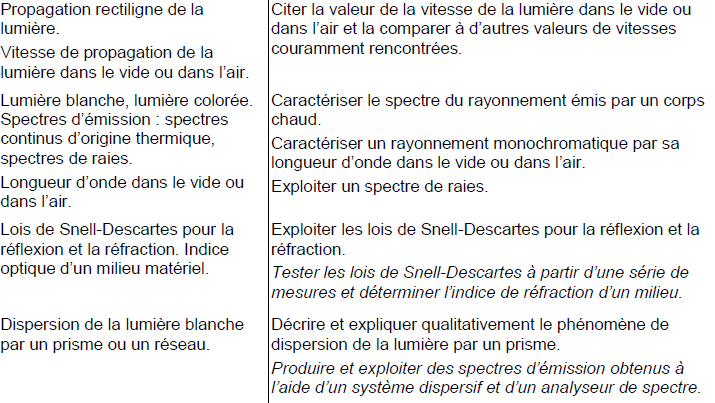
\includegraphics[width=1\textwidth]{BO.png}
\end{center}
}
% \begin{minipage}{.2\textwidth}
% 	
\includegraphics[width=1\textwidth]{QuizzSpectreEmission.png}
% 	\captionof{figure}{Quiz 1: Les spectres d'émission \\
% 	\url{https://forms.office.com/r/73PFkHSL2s}}
% 	
\includegraphics[width=1\textwidth]{Quiz2LumiereBlanche.png}

% 	
\includegraphics[width=1\textwidth]{Quiz3SnellDescartes.png}

% 	
\includegraphics[width=1\textwidth]{Quiz4Refraction.png}
% \end{minipage}


\doc{2}{Exercices dans le livre scolaire}{
		\begin{enumerate}
			\item Émission et spectre de la lumière : 9,10 p.278 et 14p.279 ainsi que 20p281.
			\item Propagation de la lumière : 10 p. 295, 27p. 299, activité star wars.
		\end{enumerate}
}
	\noindent \textbf{Quiz sur la lumière et les spectres}
\begin{figure}[ht]
	\centering
	\subfloat[Quiz 1 : Les spectres d'emission \hfill \url{https://forms.office.com/r/73PFkHSL2s}]{
\includegraphics[width=.2\textwidth]{QuizzSpectreEmission.png}}\hfill
	\subfloat[Quiz 2 : La lumière blanche \url{https://forms.office.com/r/Y5KLtYwWax}]{
\includegraphics[width=.2\textwidth]{Quiz2LumiereBlanche.png}}\hfill
	\subfloat[Quiz 3 : Propagation de la lumière \url{https://forms.office.com/r/hsJ9rJSSjL}]{
\includegraphics[width=.2\textwidth]{Quiz3SnellDescartes.png}}\hfill
	\subfloat[Quiz 4 : Déterminer un indice de réfraction \url{https://forms.office.com/r/8rFUN6Cxar}]{
\includegraphics[width=.2\textwidth]{Quiz4Refraction.png}}\hfill

\end{figure}

\clearpage
\section*{Introduction}

Les phénomènes lumineux sont omniprésents autour de nous. Mais qu’est-ce que
la lumière ? Comment peut-elle prendre des couleurs différentes ? Dans ce chapitre,
on s’intéresse à la nature et à la production de la lumière.

\begin{figure}[ht]
	\centering
	\includegraphics*[width=.43\textwidth]{Volcan.png}\hspace{1cm}
	\includegraphics*[width=.29\textwidth]{LightSky.png}
	\caption{Lave issue d'un volcan et les étoiles visibles la nuit émettent de la lumière, mais ces sources sont a priori différentes.}
\end{figure}
\vspace{-1cm}
\section{La lumière, une onde qui se propage}

\begin{center}
\textit{reférence : le livre scolaire p.275}
\end{center}

Dans le cadre du modèle ondulatoire, on considère que la lumière est une \textbf{onde} qui se \textbf{propage}. On peut caractériser une onde par sa longueur d'onde.

% \begin{figure}[ht]
% 	\centering

% \begin{tikzpicture}[x={(-150:0.7)}, y={(90:1.0)}, z={(-15:8mm)}]
% 	% Wave Function
% 	\def\wave{
% 		\draw[fill, very thick, fill opacity=0]
% 			 (0,0) sin (1,1) cos (2,0) sin (3,-1) cos (4,0)
% 				   sin (5,1) cos (6,0) sin (7,-1) cos (8,0)
% 				   sin (9,1) cos (10,0) sin (11,-1) cos (12,0);
			 
% 		\foreach \shift in {0,4,8}
% 		{
% 			\begin{scope}[xshift=\shift cm,thin]
% 					\draw[-stealth, very thick] (.5,0)  -- (0.5,0 |- 45:1cm);
% 					\draw[-stealth, very thick] (1,0)   -- (1,1);
% 					\draw[-stealth, very thick] (1.5,0) -- (1.5,0 |- 45:1cm);
% 					\draw[-stealth, very thick] (2.5,0) -- (2.5,0 |- -45:1cm);
% 					\draw[-stealth, very thick] (3,0)   -- (3,-1);
% 					\draw[-stealth, very thick] (3.5,0) -- (3.5,0 |- -45:1cm);
% 			 \end{scope}
% 		} 
% 	}
	
% 	% Red Wave
% 	\begin{scope}[canvas is zy plane at x=0, draw=blue]%, fill=red!50] 
% 		\draw[color = black, dashed] (5,1)-- (5,1.5);
% 		\draw[color = black, dashed] (9,1)-- (9,1.5);
% 		\draw [very thick, latex-latex, color = black] (5,1.5) -- (9,1.5);
% 		\draw (7,1.9) node{$\lambda$};
% 		\draw[-latex, very thick, color = black] (0,0) -- (0, 1.5) node[above]{$\textcolor{blue}{\overrightarrow{E}}$};% {$\mathbf E$};
% 		\wave
		
% 	\end{scope}
	
% 	% Blue Wave
% 	\begin{scope}[canvas is zx plane at y=0, draw=red]%, fill=cyan]
% 		%% Direction of Propagation
% 		\draw[-latex, thick, black] (0,0) -- (12.5, 0) node[rotate = -12, pos=1.15] {Direction de \\propagation};
% 		\draw[-latex, very thick, color = black] (0,0) -- (0,2) node[left] {$\textcolor{red}{\overrightarrow{B}}$};
% 		\wave
% 	\end{scope}
% 	\end{tikzpicture}
	
% 	\caption{Représentation d'une onde électromagnétique. Une telle onde est constituée d'un champ électrique $\textcolor{blue}{\overrightarrow{E}}$ et d'un champ magnétique $\textcolor{red}{\overrightarrow{B}}$ qui se propagent ensemble.}
% \end{figure}




\begin{definition}{Définition - Longueur d'onde}
	C'est une \textbf{grandeur} qui permet de décrire les \textbf{spectres lumineux}. À une radiation lumineuse monochromatique on lui associe une longueur d'onde.  On note la longueur d'onde $\lambda$ (\og{} \textit{lambda} \fg{}). Celle-ci se mesure souvent en \textbf{nanomètres} ($10^{-9}$ mètres).
	% La longueur d'onde est une période spatiale des oscillations. C'est la distance parcourue par l'onde pendant une période d'oscillation.
\end{definition}

\subsection{La célérité de la lumière une constante universelle}

Dans le vide, les ondes électromagnétiques (dont la lumière fait partie) se propagent toutes à la \textbf{même vitesse}. On note $c$ cette vitesse et on l'appelle souvent \textit{célérité}.

% \begin{mdframed}[style=prop, leftmargin=0pt, rightmargin=0pt, innertopmargin=8pt, innerbottommargin=8pt, innerrightmargin=10pt, innerleftmargin=10pt]
	\begin{Proposition}{Propriété - Vitesse de propagation de la lumière}
	% \textbf{}
		
	La célérité de la lumière dans le vide et dans l'air est égale à 
	\[c=299~792~458~\rm m\cdot s^{-1}\]
% \end{mdframed}
	\end{Proposition}

Pour les applications numériques, il est courant de prendre une valeur arrondie: 
\[c = 3,00\times 10^8 ~\rm m\cdot s^{-1}\]Il s'agit d'une valeur \textbf{limite}, aucun objet ou signal ne peut aller plus vite que la lumière dans le vide et dans l'air.

\exo{1}{La vitesse de la lumière}{
	Le Soleil est situé à environ 150 millions de kilomètres de la Terre. Quel est le temps de trajet de la lumière du Soleil à la Terre ?\bigskip

	\textbf{Solution : } $\Delta t = \dfrac{d}{v}$ A.N.: $\Delta t = \dfrac{150\times 10^6\times 10^{3}}{3,00\times 10^8} \approx 186 ~\rm s$. Le temps de trajet entre le Soleil et la Terre pour un rayon lumineux est de 186 secondes. 
	% \noindent \dotfill
}

\subsection{L'oeil humain est capable de voir certaines ondes lumineuses}

L'\oe il humain ne peut pas percevoir toutes les ondes lumineuses. Seules certaines longueurs d'ondes peuvent être détectées : c'est \textbf{le domaine du visible}. Comment appelle-t-on la grandeur qui permet de différencier les différentes ondes électromagnétiques, préciser son unité:\bigskip 

\textbf{La grandeur qui permet de différencier les ondes lumineuses est la longueur d'onde, notée $\lambda$. Cette grandeur est mesurée en nanomètres (nm)}. À chaque longueur d'onde correspond une couleur et une onde lumineuse.\bigskip

% \noindent\dotfill \bigskip

% \noindent\dotfill

L'\oe il humain est capable de distinguer seulement une petite partie des ondes électromagnétiques : c'est la lumière visible. Dans quel domaine se situe la lumière visible ?\bigskip 

\textbf{Le domaine visible s'étend entre 400 et 800 nm.}\bigskip

% \noindent \dotfill \bigskip

% \noindent \dotfill

\begin{definition}{Définition - la couleur}
	La couleur est la perception subjective qu'a l'\oe il d'une ou de plusieurs longueurs d'ondes lumineuses. À \textbf{chaque longueur d'onde} dans le domaine du visible est \textbf{associée une radiation monochromatique}, c'est à dire une couleur.
\end{definition}
% \clearpage

\subsection{La lumière blanche, une onde lumineuse polychromatique}

La lumière blanche est constituée d'un mélange de toutes les longueurs d'ondes (de toutes les couleurs). Il n'existe pas de longueur d'onde unique associée à la lumière blanche.\bigskip

\begin{center}
On parle alors de lumière \textbf{polychromatique}%\makebox[5cm]{\dotfill}.
\end{center}

Il est possible de représenter la \textbf{composition de la lumière} par un diagramme appelé \textbf{spectre}, dont l'échelle est la longueur d'onde.

\begin{figure}[ht]
	\centering
	% \begin{tikzpicture}
	\pgfspectra[width=.9\textwidth, height = 2cm, axis,axis step = 20, begin = 380, end = 780,axis font= \footnotesize, axis color=black!0, axis font color=black, axis label text ={$\lambda$ (nm)} ]%\fontsize{3}{3}\itshape\selectfont]
	% \end{tikzpicture}
	\caption{Spectre de la lumière blanche dans le domaine du visible}
\end{figure}

\exo{2}{Éclairage routier}{Les lampes utilisées pour l'éclairage routier émettent de la lumière dont la longueur d'onde est $\lambda = 589 \rm nm$. Cette lumière est-elle visible ? Quelle est sa couleur ? \bigskip

\textbf{Solution : } Oui cette lumière est visible. Elle correspond à la couleur orange d'après le spectre de la lumière de la figure 2.
% \noindent \dotfill \bigskip

% \noindent \dotfill

}


\section{Émission de la lumière}
\begin{center}
\textit{reférence : le livre scolaire p.275}
\end{center}

Comme nous l'avons vu en introduction, il existe une grande variété de sources lumineuses. On se proposer d'étudier deux types d'émission lumineuses : l'émission de lumière par un corps chaud et l'émission de lumière par une entité chimique.

\subsection{La lumière émise par un corps dépend de sa température}

Tous les corps émettent naturellement de la lumière. La nature de cette lumière dépend de la \textbf{température} du corps : si un corps est suffisamment chauffé, il peut se mettre à rayonner de la \textbf{lumière visible.} Cette lumière est constituée d'une \textbf{infinité de couleurs} (d'intensités différentes) : on dit que son spectre est \textbf{polychromatique et continu}.

\begin{figure}[ht]
	\centering
	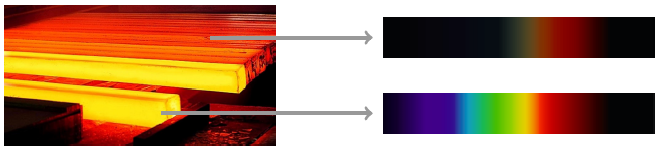
\includegraphics[width=1\textwidth]{EmissionCorpschaud.png}
	\caption{Allure des spectres des lumières émises par des barres d'acier chauffées à des températures différentes.}
\end{figure}

\begin{Proposition}{Propriété - Lumière émise par un corps chaud}
	\bigskip

	Plus la température de surface d'un corps augmente, plus son maximum d'intensité lumineuse émise se déplace vers les courtes longueurs d'onde (vers le bleu). À l'inverse, lorsqu'un corps se refroidit, il émet un rayonnement porté vers les longueurs d'onde les plus grandes (vers le rouge).
	% \noindent\dotfill \bigskip

	% \noindent\dotfill \bigskip

	% \noindent\dotfill %\bigskip

	% \noindent\dotfill 	
\end{Proposition}


% \begin{Exercice}{Exercice 3 - Température des étoiles}
\exo{3}{La température des étoiles}{
	Les photographies ci-dessous montrent les étoiles \textit{Bellatrix} (à gauche) et \textit{Bételgeuse} (à droite). Laquelle de ces deux est la plus chaude ? 

	\begin{center}
	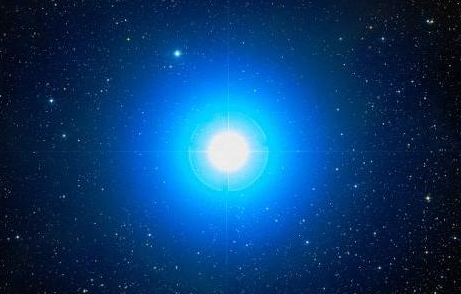
\includegraphics[width=.3\textwidth]{Bellatrix.png}\hspace{1cm}
	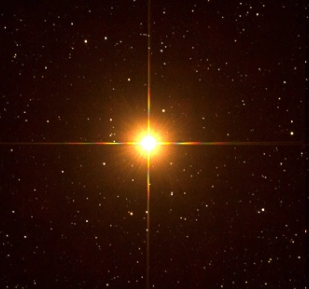
\includegraphics[width=.2\textwidth]{Betelgeuse.png}\bigskip
\end{center}
	\textbf{Solution :} L'étoile la plus chaude est celle qui émet au maximum dans le rayonnement bleu c'est à dire l'étoile appelée Bellatrix.
	% \dotfill \bigskip

	% \dotfill
}
\clearpage
\subsection{Spectre de la lumière d'une entité chimique, un code barre des atomes}

Lorsqu'une entité chimique (atome, ion ou molécule) est excitée, celle-ci peut \textbf{émettre de la lumière}

\begin{figure}[ht]
	\centering
	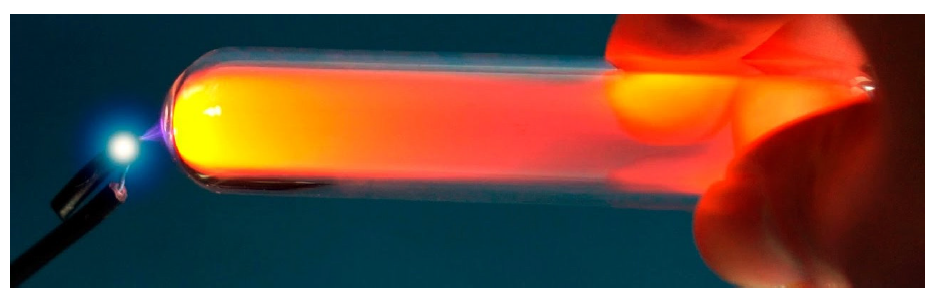
\includegraphics[width=.6\textwidth]{Neon.png}
	\caption{Ampoule contenant du néon excitée par un arc électrique : le gaz émet de la lumière rouge.}
\end{figure}

Inversement, une entité peut \textbf{absorber de la lumière} (la même que celle qu'elle émet) lorsqu'on éclaire. On peut ainsi représenter \textbf{les spectres d'emission} et \textbf{d'absoprtion} d'une entité chimique donnée. Ces spectres ne contiennent que certaines couleurs, appelées \textbf{raies spectrales} : on dit qu'ils sont \textbf{discontinus}.


\begin{figure}[ht]
	\centering
	\pgfspectra[element = Ne, width=.9\textwidth, height = 2cm]\\%\fontsize{3}{3}\itshape\selectfont]\\

	\pgfspectra[element = Ne, absorption, width=.9\textwidth, height = 2cm, axis,axis step = 20, begin = 380, end = 780,axis font= \footnotesize, axis color=black!0, axis font color=black,axis label text ={$\lambda$ (nm)}]%\fontsize{3}{3}\itshape\selectfont]
	\caption{Spectres d'émission (en haut) et d'absorption (en bas) du néon \isotope{20}{10}{Ne}}
\end{figure}

\begin{Proposition}{Propriété - Spectre d'une entité chimique}

	Les spectres d'emission ou d'absorption sont caractéristiques d'une seule et même entité chimique. 
	% \bigskip

	% \noindent\dotfill \bigskip

	% \noindent\dotfill \bigskip

	% \noindent\dotfill \bigskip
\end{Proposition}

\clearpage
\section{Propagation de la lumière}

\begin{center}
	\textit{référence : le livre scolaire p. 291-292}
\end{center}

Les phénomènes lumineux, comme la réflexion d'objets sur la surface d'un lac ou l'illusion d'optique d'un crayon brisé lorsqu'il est plongé dans un verre d'eau sont omniprésents autout de nous. Dans cette partie on s'intéresse à la \textbf{propagation de la lumière}. 

\begin{figure}[ht]
	\centering
	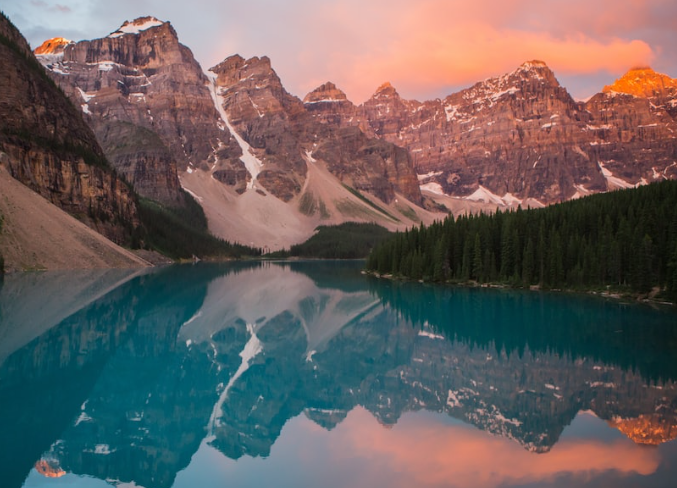
\includegraphics[width=.4\textwidth]{montagnesreflets.png}\hspace{2.5cm}
	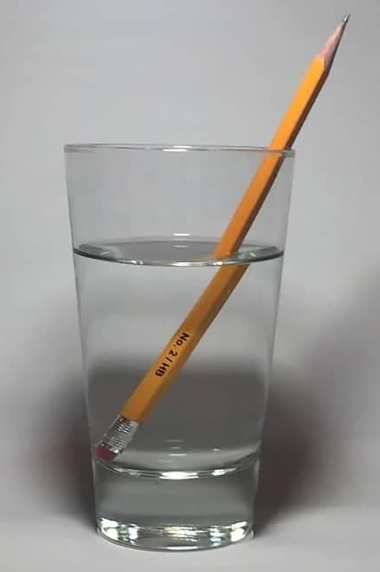
\includegraphics[width=.2\textwidth]{crayon.png}
	\caption{Phénomène lié à la propagation de la lumière au voisinage d'interfaces air-eau.}
\end{figure}

\subsection{Propagation d'une lumière monochromatique}

On s'intéresse dans un premier temps aux lumières \textbf{monochromatiques}, c'est-à-dire\medskip

ne comportant qu'une seule \textbf{longueur d'onde ou couleur}.%\dotfill

\begin{definition}{Définition - Rayon lumineux}

C'est une notion d'\textbf{optique} et un outil mathématique qui permet de décrire le trajet de la lumière de manière simple. On représente un rayon lumineux par une droite munie d'une flèche. 
% \bigskip

% \noindent\dotfill \bigskip

% \noindent \dotfill \bigskip
\end{definition}
\subsubsection{Milieu transparent et homogène}

Lorsque la lumière se propage dans un milieu (air, verre, eau,...) elle intéragit avec celui-ci. Ce dernier modifie les propriétés de la lumière. Il peut changer sa vitessem lui prendre de l'énergie. Dans cette partie on considère que la lumière se propage dans un milieu \textbf{transparent} et \textbf{homogène}. 
\begin{definition}{Définition - Transparent}
Un milieu \textbf{transparent} est un milieu où les ondes électromagnétiques comme la lumière ne sont pas absorbées. Autrement dit elles ne vont pas perdre en intensité.

	% \bigskip
	
	% \noindent\dotfill \bigskip
	
	% \noindent \dotfill \bigskip
\end{definition}

\textbf{Exemple : } les lunettes de soleil sont un milieu qui n'est pas transparent. Elles permettent d'absorber la lumière du soleil pour ne pas abimer les yeux.

\begin{definition}{Définition - Homogène}
	Un milieu \textbf{homogène} est un milieu qui a la même composition et les mêmes caractéristiques en tout point de l'espace.
		% \bigskip
		
		% \noindent\dotfill \bigskip
		
		% \noindent \dotfill \bigskip

		% \noindent \dotfill
\end{definition}
\clearpage
\begin{figure}[ht]
	\centering
	\begin{minipage}{.45\textwidth}
		\centering
	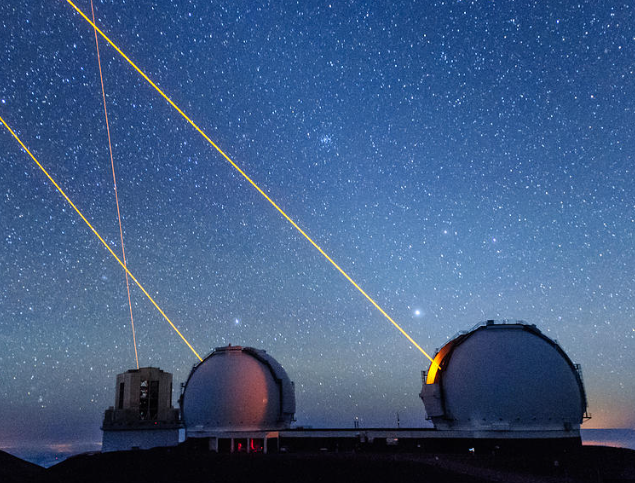
\includegraphics[width=.8\textwidth]{LaserParty.png}
	\end{minipage}\hspace{2cm}
	\begin{minipage}{.4\textwidth}
	\caption{Rayon LASER utilisé par des astronomes à Manua Kea sur l'île de Hawai pour pointer des étoiles du ciel.}
	\end{minipage}
\end{figure}

\begin{Proposition}{Propriétés - Propagation dans un milieu transparent et homogène}
	Dans un milieu \textbf{homogène} et \textbf{transparent} la lumière se propage en ligne droite.
	
	% \bigskip

	% \noindent\dotfill \bigskip

	% \noindent \dotfill 
\end{Proposition}

\subsection{Propagation à l'interface entre deux milieux}

On considère maintenant que la lumière arrive sur une \textbf{interface séparant deux milieux} homogènes et transparents. 

\begin{Proposition}{Propriétés - Première loi de Snell-Descartes}
	
	Les rayons incident, réfléchi et réfracté appartiennent au même plan : \textbf{le plan d'incidence}.
	
	% \medskip 

	% \dotfill \medskip
	
	% \dotfill
\end{Proposition}

\begin{figure}[ht]
	\centering
	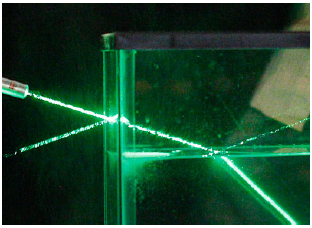
\includegraphics[width=.32\textwidth]{RayonLaser.png}\hspace{2cm}
	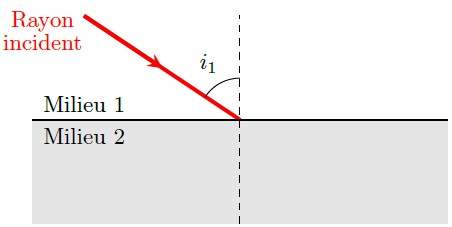
\includegraphics[width=.42\textwidth]{RayonIncident.png}
	\caption{Rayon incident sur une interface entre deux milieux 1 et 2. Compléter le schéma lorsque le rayon du laser passe de l'air à l'eau.}
\end{figure}

Un rayon lumineux arrivant à la frontière entre deux milieux peut :
\begin{itemize}
	\item Changer de direction et rester dans le même milieu; c'est la \textbf{réflexion}.
	\item Changer de direction et changer de milieu; c'est la \textbf{réfraction}. 
\end{itemize}

\exo{4}{Phénomène lumineux aux interfaces}{
	Donner le nom de chaque phénomène représenté ci-dessous.
	\begin{center}
	\begin{tikzpicture}[scale = 1.2]
		% \draw[dashed] (1.5,-1.5) -- (1.5,1.5);
		\draw[color = white, fill = cyan!30] (0,0) rectangle ++ (3,1);
		\draw[dashed] (1.5,0) -- (1.5,2);
		\draw[very thick, color = red, postaction={on each segment={mid arrow=red}}] (.5,2) -- (1.5,1);
		\draw[very thick, color = red, -latex] (1.5,1) --(2.5 ,2);
		\draw (0.3,.7) node{Eau};
		\draw (0.3,1.2) node{Air};
		\draw (1.5,1.7) arc (90:135:.7) node[above]{$i_{1}$};
		\draw [very thick] (0,1) -- (3,1);
		\draw (1.5,-.2) node{la réflexion};
		\draw[dashed] (3,-.5)-- (0,-.5);
	\end{tikzpicture}\hspace{2cm}
	\begin{tikzpicture}[scale = 1.2]
		% \draw[dashed] (1.5,-1.5) -- (1.5,1.5);
		\draw[color = white, fill = cyan!30] (0,0) rectangle ++ (3,1);
		\draw[dashed] (1.5,0) -- (1.5,2);
		\draw[very thick, color = red, postaction={on each segment={mid arrow=red}}] (.5,2) -- (1.5,1);
		\draw[very thick, color = red, -latex] (1.5,1) --(2 ,.2);
		\draw (0.3,.7) node{Eau};
		\draw (0.3,1.2) node{Air};
		\draw (1.5,1.7) arc (90:135:.7) node[above]{$i_{1}$};
		\draw [very thick] (0,1) -- (3,1);
		\draw (1.5,-.2) node{la réfraction};
		\draw[dashed] (0,-.5) -- (3,-.5);
	\end{tikzpicture}
\end{center}
}

\subsubsection{Réfraction}

Il existe des lois permettant de \textbf{prévoir} les angles que font les rayons textbf{réfléchis} (noté $r$) et \textbf{réfractés} (notés $ i_{2}$). Ce sont les lois énoncées par Willebrord \bsc{Snell} et René \bsc{Descartes} au XVII$^{\rm e}$ siècle.\medskip

\begin{minipage}{.6\textwidth}
\begin{Proposition}{Propriété - Loi de \bsc{Snell-Descartes} pour la réfraction}
	La loi de \bsc{Snell-Descartes} pour la réfraction s'écrit : 

	\begin{equation}
		n_1\sin(i_1) = n_2\sin(i_2)
	\end{equation}
	
	avec $n_1$ l'indice optique pour le milieu 1 et $n_2$ pour le milieu 2. $i_1$ et $i_2$ sont les angles incident et réfracté. 
	% \bigskip

	% \dotfill\bigskip

	% \dotfill\bigskip

	% \dotfill
\end{Proposition}

L'angle que que fait le rayon réfracté avec la normale dépend des milieux, que l'on caractérise à l'aide de l'\textbf{indice optique}. Quelques valeurs d'indices optiques sont répertoriées dans le tableau ci-contre.
\end{minipage}
\begin{minipage}{.4\textwidth}
% \begin{table}[ht]
	\centering
	\begin{tabular}{|c|c|}
		\hline
		\textbf{Milieu} & \textbf{indice optique} \\ \hline
		Vide  			& 1 (exactement) \\ \hline
		Air				& 1,00  \\ \hline
		Verre           & $\sim 1.50$ \\ \hline
		Eau				& $1,33$ \\ \hline
		Diamant 		& 2,5 \\ \hline
	\end{tabular}
% \end{table}
\end{minipage}
\exo{5}{La réfraction}{
	Un rayon de soleil atteint une vitre en faisant un angle de 30$^\circ$ avec la normale de la vitre. 
	\begin{enumerate}
		\item Représenter la situation par un schéma.
		\begin{center}
			\begin{tikzpicture}
				\draw[step = 0.5, color = black!10] (0,0) grid++ (10,5);
					\draw[color = white, fill = cyan!30] (0,0) rectangle ++ (10,2);
					\draw[thick, dashed] (5,0) -- (5,5);
					\draw[ultra thick, color = red, postaction={on each segment={mid arrow=red}}] (3,5) -- (5,2.5);
					\draw[thick] (5,4) arc (90:120:2) node[above, midway]{$\boldsymbol{i_1}$};
					\draw[ultra thick, color = red, postaction={on each segment={mid arrow=red}}] (5,2.5) --(6 ,0);
					\draw (0.9,4) node{Milieu 1 :};
					\draw (1.2,3.5) node{Air, $n_1=1,0$};
					\draw (0.9,1.8) node{Milieu 2 : };
					\draw (1.2,1.3) node{verre, $n_2=1.5$};
					\draw [very thick] (0,2.5) -- (9,2.5);
					\draw[thick] (5,1) arc (-90:-78:2.5) node[below, midway]{$\boldsymbol{i_2}$};
			\end{tikzpicture}
			% {\large \textit{SCHEMA À COMPLETER SUR LA FEUILLE }}
	\end{center}
		\item Quel angle fait le rayon  réfracté avec la normale de la vitre ? À l'aide de la loi de \bsc{Snell-Descartes} :
		
		\begin{equation}
			n_1\sin(i_1) = n_2\sin(i_2)
		\end{equation}

		Soit $\sin(i_2) = \dfrac{n_1}{n_2}\sin(i_1)$  A.N. : $\sin(i_2)=0.3$. 

		Et $i_2 = \arcsin(sin(i_2))$ A.N.: $i_2 = 0.34~ \rm radians = 19~ \rm degrés$

		% \noindent \dotfill \medskip

		
		% \noindent \dotfill \medskip

		
		% \noindent \dotfill \medskip

	\end{enumerate}
}
\vspace{-.2cm}
\subsubsection{Réflexion}
\begin{Proposition}{Propriété - Loi de \bsc{Snell-Descartes} pour la réflexion}
	
	La loi de \bsc{Snell-Descartes} pour la réflexion dit que l'angle entre la normale et le rayon réfléchi noté $r$ est égal à l'angle incident $i_1$ : $r=i_1$
	% \bigskip

	% \dotfill\bigskip 

	% \dotfill \bigskip

	% \dotfill \bigskip

	% \dotfill
	
\end{Proposition}

\clearpage
\subsection{Dispersion d'une lumière polychromatique}

On considère dans cette partie la dispersion d'une \textbf{lumière polychromatique}. Pour disperser une lumière polychromatique il faut utiliser un milieu dispersif comme un \textbf{prisme}.

\begin{figure}[ht]
	\centering
	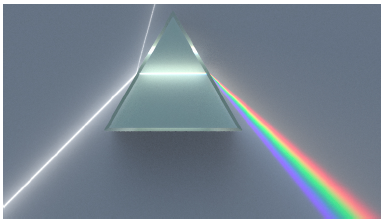
\includegraphics[width=.42\textwidth]{prisme.png}\hspace{1cm}
	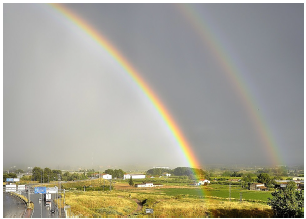
\includegraphics[width=.38\textwidth]{DoubleArcEnCiel.png}
	\caption{À gauche un rayon lumineux est réfracté deux fois en traversant un prisme en verre. La lumière blanche est décomposée en différente couleurs. À droite une photo d'un double arc-en-ciel.}
\end{figure}

\begin{definition}{Définition - Dispersion}
	La dispersion de la lumière c'est le phénomène affectant une onde électromagnétique se propageant dans un milieu dispersif. C'est ce phénomène qui explique la décomposition de la lumière blanche lorsqu'elle traverse un prisme.\medskip
\end{definition}\bigskip


\begin{definition}{Définition - Milieu dispersif}
	Un milieu est dit dispersif si la vitesse de propagation de l'onde dépend de la longeur d'onde $\lambda$ du rayonnement qui la traverse.\medskip

	Dans un milieu différent, on note la vitesse $v$. L'indice d'un milieu est une grandeur sans unité, et la relation qui relie $n,c$ et $v$ est : 
	\begin{equation}
		n = \dfrac{c}{v}.
	\end{equation}
	$n\leq 1$ car $c$ la célérité de la lumière est une vitesse limite dans l'univers qui ne peut pas être dépassée.
\end{definition}


On a vu qu'un prisme en verre flint (TP) permet de décomposer la lumière en plusieurs couleurs. Dans le verre flint l'indice de réfraction est différent pour chaque longueur d'onde. Donc les angles de réfraction sont différents pour chaque rayonnement. Les rayonnements sont alors séparés et forment un spectre lumineux.
	
\clearpage

\exo{6}{L'arc-en-ciel}{
	\begin{enumerate}
		\item Par quel temps les arcs-en-ciel apparaissent-ils habituellement ?\bigskip
		
		Il faut un temps humide avec du soleil, après une averse par exemple c'est idéal.

		\item À votre avis, quel milieu est responsable de la dispersion de la lumière dans ce cas ? Que dit-on de ce type de milieux ? 
		
		Ce sont les gouttes d'eau dispersées dans l'atmosphère qui permettent de disperser les rayons lumineux provenant du soleil. L'eau est donc un milieu dispersif.

		\item L'air est-il un milieu dispersif ?
		
		L'air sec, n'est pas un milieu dispersif, c'est un milieu homogène et transparent. En revanche un air humide n'est pas homogène, il devient dispersif.

		\item Lorsque les conditions sont favorables, il est possible d'observer deux arcs-en-ciel (voir photo). Comment cela-est-il possible ?
		
		Le double arc-en-ciel est provoqué par une double réfléxion de la lumière du soleil à l'intérieur des gouttes de pluie. Il apparaît alors dans la direction opposée au soleil.
	\end{enumerate}
}

\begin{figure}[ht]
	\centering
	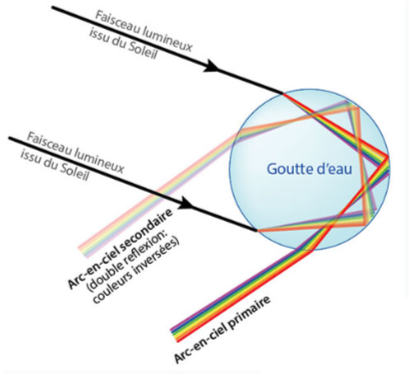
\includegraphics[width=.8\textwidth]{Double Arc-en-ciel.jpg}
	\caption{Double réflexion dans une goutte d'eau}
\end{figure}
\end{document}

%%
%% FIN DU DOCUMENT
%%
